\section{Systematic-aggregation audit: the panel is genetically concentrated on pancreatic cancer (Open Targets)}
The previous three audits found no pancreatic specificity for the panel at the
germline (gnomAD), expression (GTEx), or curated clinical-evidence (CIViC)
levels. Here we ask whether \emph{systematic cross-datasource aggregation}
agrees, using the Open Targets Platform GraphQL API. We retrieved the complete
target--disease association tables for exocrine pancreatic carcinoma
(MONDO\_0005192, 11,589 targets), breast cancer (MONDO\_0007254, 17,252), and
myeloproliferative disorder (EFO\_0004251, 13,488) --- every row carries an
Ensembl gene identifier, an overall association score, and per-datasource
component scores (19 datasources seen) --- plus the
tractability and drug-candidate records of the six audit genes
(\texttt{results/opentargets\_assoc\_rows.csv}, one row per association
record).

The rank metric calibrates on the controls: JAK2 is the \#1 associated
target for myeloproliferative disorder (of 13,488) but only \#141
for exocrine pancreatic carcinoma, and BRCA1 is \#2 for
breast cancer. Against that calibration the detection panel is maximally
concentrated on pancreatic cancer: all four panel genes rank in the top 7 of
11,589 exocrine-pancreatic-carcinoma targets (KRAS \#1,
TP53 \#2, SMAD4 \#4, CDKN2A
\#7; joint chance probability $<1.3e-13$
under uniform placement), and each ranks markedly worse in the two control
diseases (Table~\ref{tab:opentargets}). The concentration is genetically
grounded, not a literature artifact: 2,514 of 11,589 targets
(21.7\%, 95\% CI 21.0--22.5\%) are literature-only
(Europe PMC score $\ge0.25$ with every genetic datasource $<0.25$), but only
5 of the top 100 are literature-only versus 21.8\% of the
remainder (Fisher $p=7.1e-06$), and every
panel gene carries strong genetic-datasource support (max genetic score
$\ge0.92$).

\begin{table}[h]\centering\footnotesize
\begin{tabular}{@{}lllllp{5.6cm}@{}}
\hline
Gene & group & pancreatic & breast & MPN & drug candidates \\ \hline
KRAS & panel & \#1 & \#33 & \#20 & 3: 2 approval, 1 phase 2 \\
TP53 & panel & \#2 & \#7 & \#26 & 9: 5 phase 3, 4 phase 2 \\
CDKN2A & panel & \#7 & \#88 & \#221 & none (direct-target) \\
SMAD4 & panel & \#4 & \#357 & \#608 & none (direct-target) \\
BRCA1 & breast control & \#9 & \#2 & \#352 & none (direct-target) \\
JAK2 & mpn control & \#141 & \#329 & \#1 & 31: 12 approval, 6 phase 4, 3 phase 3, 1 phase 2 3, 6 phase 2, 1 phase 1 2, 2 phase 1 \\
\hline
\end{tabular}
\caption{Open Targets association ranks (of 11,589 / 17,252 / 13,488 targets per
disease) and direct-target drug candidates. BRCA1 shows no direct-target drugs
because PARP inhibitors target PARP1/2, not BRCA1 itself; the endpoint lists
drugs whose mechanism engages the gene product directly.}
\label{tab:opentargets}
\end{table}

The pharmacology is consistent with the genetics. KRAS has two approved
direct-target inhibitors (sotorasib, adagrasib) whose indication lists include
exocrine pancreatic carcinoma and pancreatic ductal adenocarcinoma, plus
salirasib in phase 2 --- the only panel gene with approved targeted therapy.
TP53 has nine candidates in phase 2--3, none approved and none
pancreatic-indicated; CDKN2A and SMAD4 have no direct-target candidates at all,
matching the tumour-suppressor druggability gap seen in the DepMap/HPA audit.
The JAK2 control shows the converse pattern: 31 direct-target candidates
(12 approved) whose pancreatic rows (ruxolitinib, momelotinib, tofacitinib)
reflect trial history in a non-canonical indication.

\begin{figure}[h]\centering
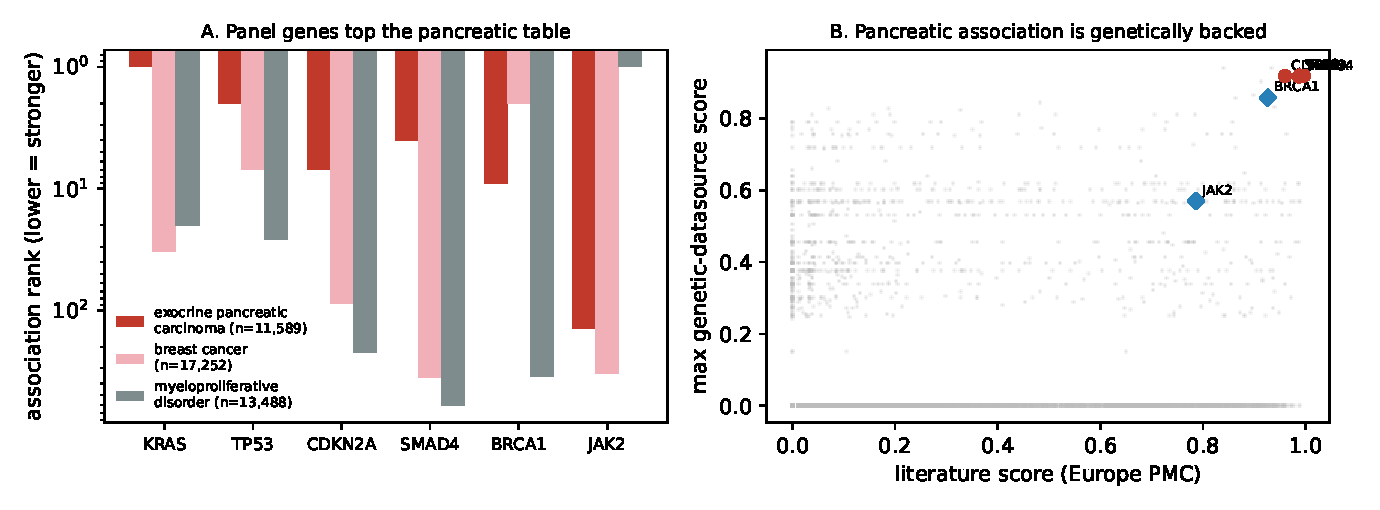
\includegraphics[width=0.98\linewidth]{figs/fig_opentargets.pdf}
\caption{(A) Association rank of the six audit genes in the three disease
tables (log scale, inverted; lower = stronger). (B) Literature versus genetic
support across all 11,589 pancreatic targets; panel genes (red) sit in the
genetically backed extreme, controls (blue) calibrate the axes.}
\end{figure}

Reconciled with the CIViC audit, the picture is sharp: the panel is
\emph{genetically} concentrated on pancreatic cancer (top 7 of 11,589) while
its \emph{curated clinical-evidence base} is indication-diffuse (4.2\%
pancreatic). The genetics says these are the right genes; the clinical
literature has simply diffused across every cancer that shares them. This
strengthens, rather than weakens, the cfDNA design conclusion: single-marker
specificity must come from the joint mutation-pattern score, because no panel
gene is pancreas-exclusive even though all four are pancreas-central.
